\documentclass{article}

\usepackage{url}
\usepackage{amsmath,amssymb}
\usepackage{graphicx,svg}

\begin{document}
\title{Lecture 13\\ CT System Analysis and Design using Laplace}
\author{C.L. Wyatt}
\date{\today}
\maketitle

Recall from ECE 2714 that we can analyze electrical circuits that form LTI systems by

\begin{itemize}
  \item Deriving a governing equation (LCDE)
  \item Finding the impulse response $h(t)$
  \item Using convolution to determine the output $y(t)$ given an input $x(t)$ 
\end{itemize}

Or alternatively using Fourier analysis

\begin{itemize}
  \item Determine stability and derive the frequency response $H(j \omega)$
  \item use convolution theorem to find output $Y(j\omega)$ and use the inverse Fourier transform to find $y(t)$.
\end{itemize}

Now that we have Laplace as a tool we can simplify this process further. The idea is to go back to circuits and take the Laplace transform of each element's voltage-current model

\begin{itemize}
\item Resistor 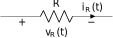
\includegraphics[alt="Voltage Current for Resistor"]{figures/fig13_1.svg}
  \begin{align*}
    v_R(t) &= R\, i_R(t)\\
    V_R(s) &= R\, I_R(s)
  \end{align*}
  Impedance $R$, Admittance $\frac{1}{R}$
  
\item Capacitor 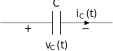
\includegraphics[alt="Voltage Current for Capacitor"]{figures/fig13_2.svg}
    \begin{align*}
    i_C(t) &= C\, \frac{dv_c}{dt}(t)\\
    I_C(s) &= C\left[sV_C(s) - v_c(0^-) \right]\\
    I_C(s) &= CsV_C(s) - Cv_c(0^-)
    \end{align*}
    or rearranging
    \[
    V_C(s) = \frac{1}{Cs}I_C(s) + \frac{v_C(0^-)}{s}
    \]
    Impedance $\frac{1}{Cs}$, Admittance $Cs$
  \item Inductor 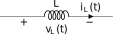
\includegraphics[alt="Voltage Current for Inductor"]{figures/fig13_3.svg}
    \begin{align*}
    v_L(t) &= L\, \frac{di_L}{dt}(t)\\
    V_L(s) &= L\left[sI_L(s) - i_L(0^-) \right]\\
    V_L(s) &= LsI_L(s) - Li_L(0^-)
    \end{align*}
    or rearranging
    \[
    I_L(s) = \frac{1}{Ls}V_L(s) + \frac{i_L(0^-)}{s}
    \]
    Impedance $Ls$, Admittance $\frac{1}{Ls}$
\end{itemize}

This gives us new circuit models in Laplace domain with either constant voltage or current sources representing the terms containing auxiliary conditions at $t=0^-$. Using KVL and KCL with these models gives us a convenient way to go from a circuit directly to a transfer function.

Example: RC with IC

Example: RLC with no I.C.

This works with active (op-amp) circuits as well.

Example: Sallen-key

Most upper level circuit courses will use these techniques. e.g. AC-circuits.

\section{Analyzing Block Diagrams}

Recall from ECE 2714 that block diagrams can be used to model systems and implement/realize systems.

\begin{figure}
  \centering
  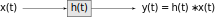
\includegraphics[alt="simple block in time domain"]{figures/fig13_4.svg}
  $\Longrightarrow$
    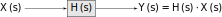
\includegraphics[alt="simple block in Laplace domain"]{figures/fig13_5.svg}
  \caption{Transformation of input and output to Laplace domain (transfer function) for a single block.}
\end{figure}

\begin{itemize}
\item series connection, the overall transfer function $H(s) = H_1(s)\cdot H_2(s)$ 
\begin{figure}
  \centering
  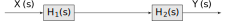
\includegraphics[alt="series connection in Laplace domain"]{figures/fig13_6.svg}
  \caption{Transformation of input and output to Laplace domain for a series connection.}
\end{figure}

\item parallel connection, the overall transfer function $H(s) = H_1(s)+ H_2(s)$ 
\begin{figure}
  \centering
  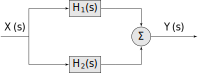
\includegraphics[alt="parallel connection in Laplace domain"]{figures/fig13_7.svg}
  \caption{Transformation of input and output to Laplace domain for a parallel connection.}
\end{figure}

\item feedback connection, the overall transfer function $H(s) = \frac{H_1(s)}{1+ H_1(s)\cdot H_2(s)}$ 
\begin{figure}
  \centering
  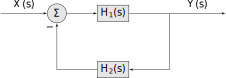
\includegraphics[alt="feedback connection in Laplace domain"]{figures/fig13_8.svg}
  \caption{Transformation of input and output to Laplace domain for a feedback connection.}
\end{figure}
\end{itemize}

We can use block diagrams to derive an overall transfer function from sub-components.

Example: PID controller

Example: DC Motor

\section{System Realization}

We can also use block diagrams in the opposite way, to implement, or realize, a given transfer function (for example from a filter design) using three basic building blocks: summation, amplifier (gain), and integrator.

\begin{figure}
  \centering
  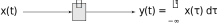
\includegraphics[alt="integrator block in time domain"]{figures/fig13_9.svg}
  $\Longrightarrow$
    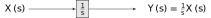
\includegraphics[alt="integrator block in Laplace domain"]{figures/fig13_10.svg}
  \caption{Transformation of an integrator to Laplace domain (transfer function).}
\end{figure}

The realization is not unique, with different canonical forms, each with
advantages and disadvantages (e.g. reduced number of components and reduced sensitivity to component variation).

\subsection{Example}

Given a transfer function

\[
H(s) = \frac{s+a}{s^2 + bs + c}
\]
for $a,b,c\in\mathbb{R}$, implement the system in terms of summations, amplifiers, and integrators.

TODO: DFI, DFII, transposed DFII, parallel and cascade of second order systems

\end{document}
